\chapter{Perancangan}
\label{chap:perancangan}

Bab ini membahas perancangan untuk seluruh fitur yang diimplementasi pada  perangkat lunak SharIF Judge.

\section{Rancangan Antarmuka}
\label{sec:4:antarmuka}

\begin{figure}[H]
	\centering  
	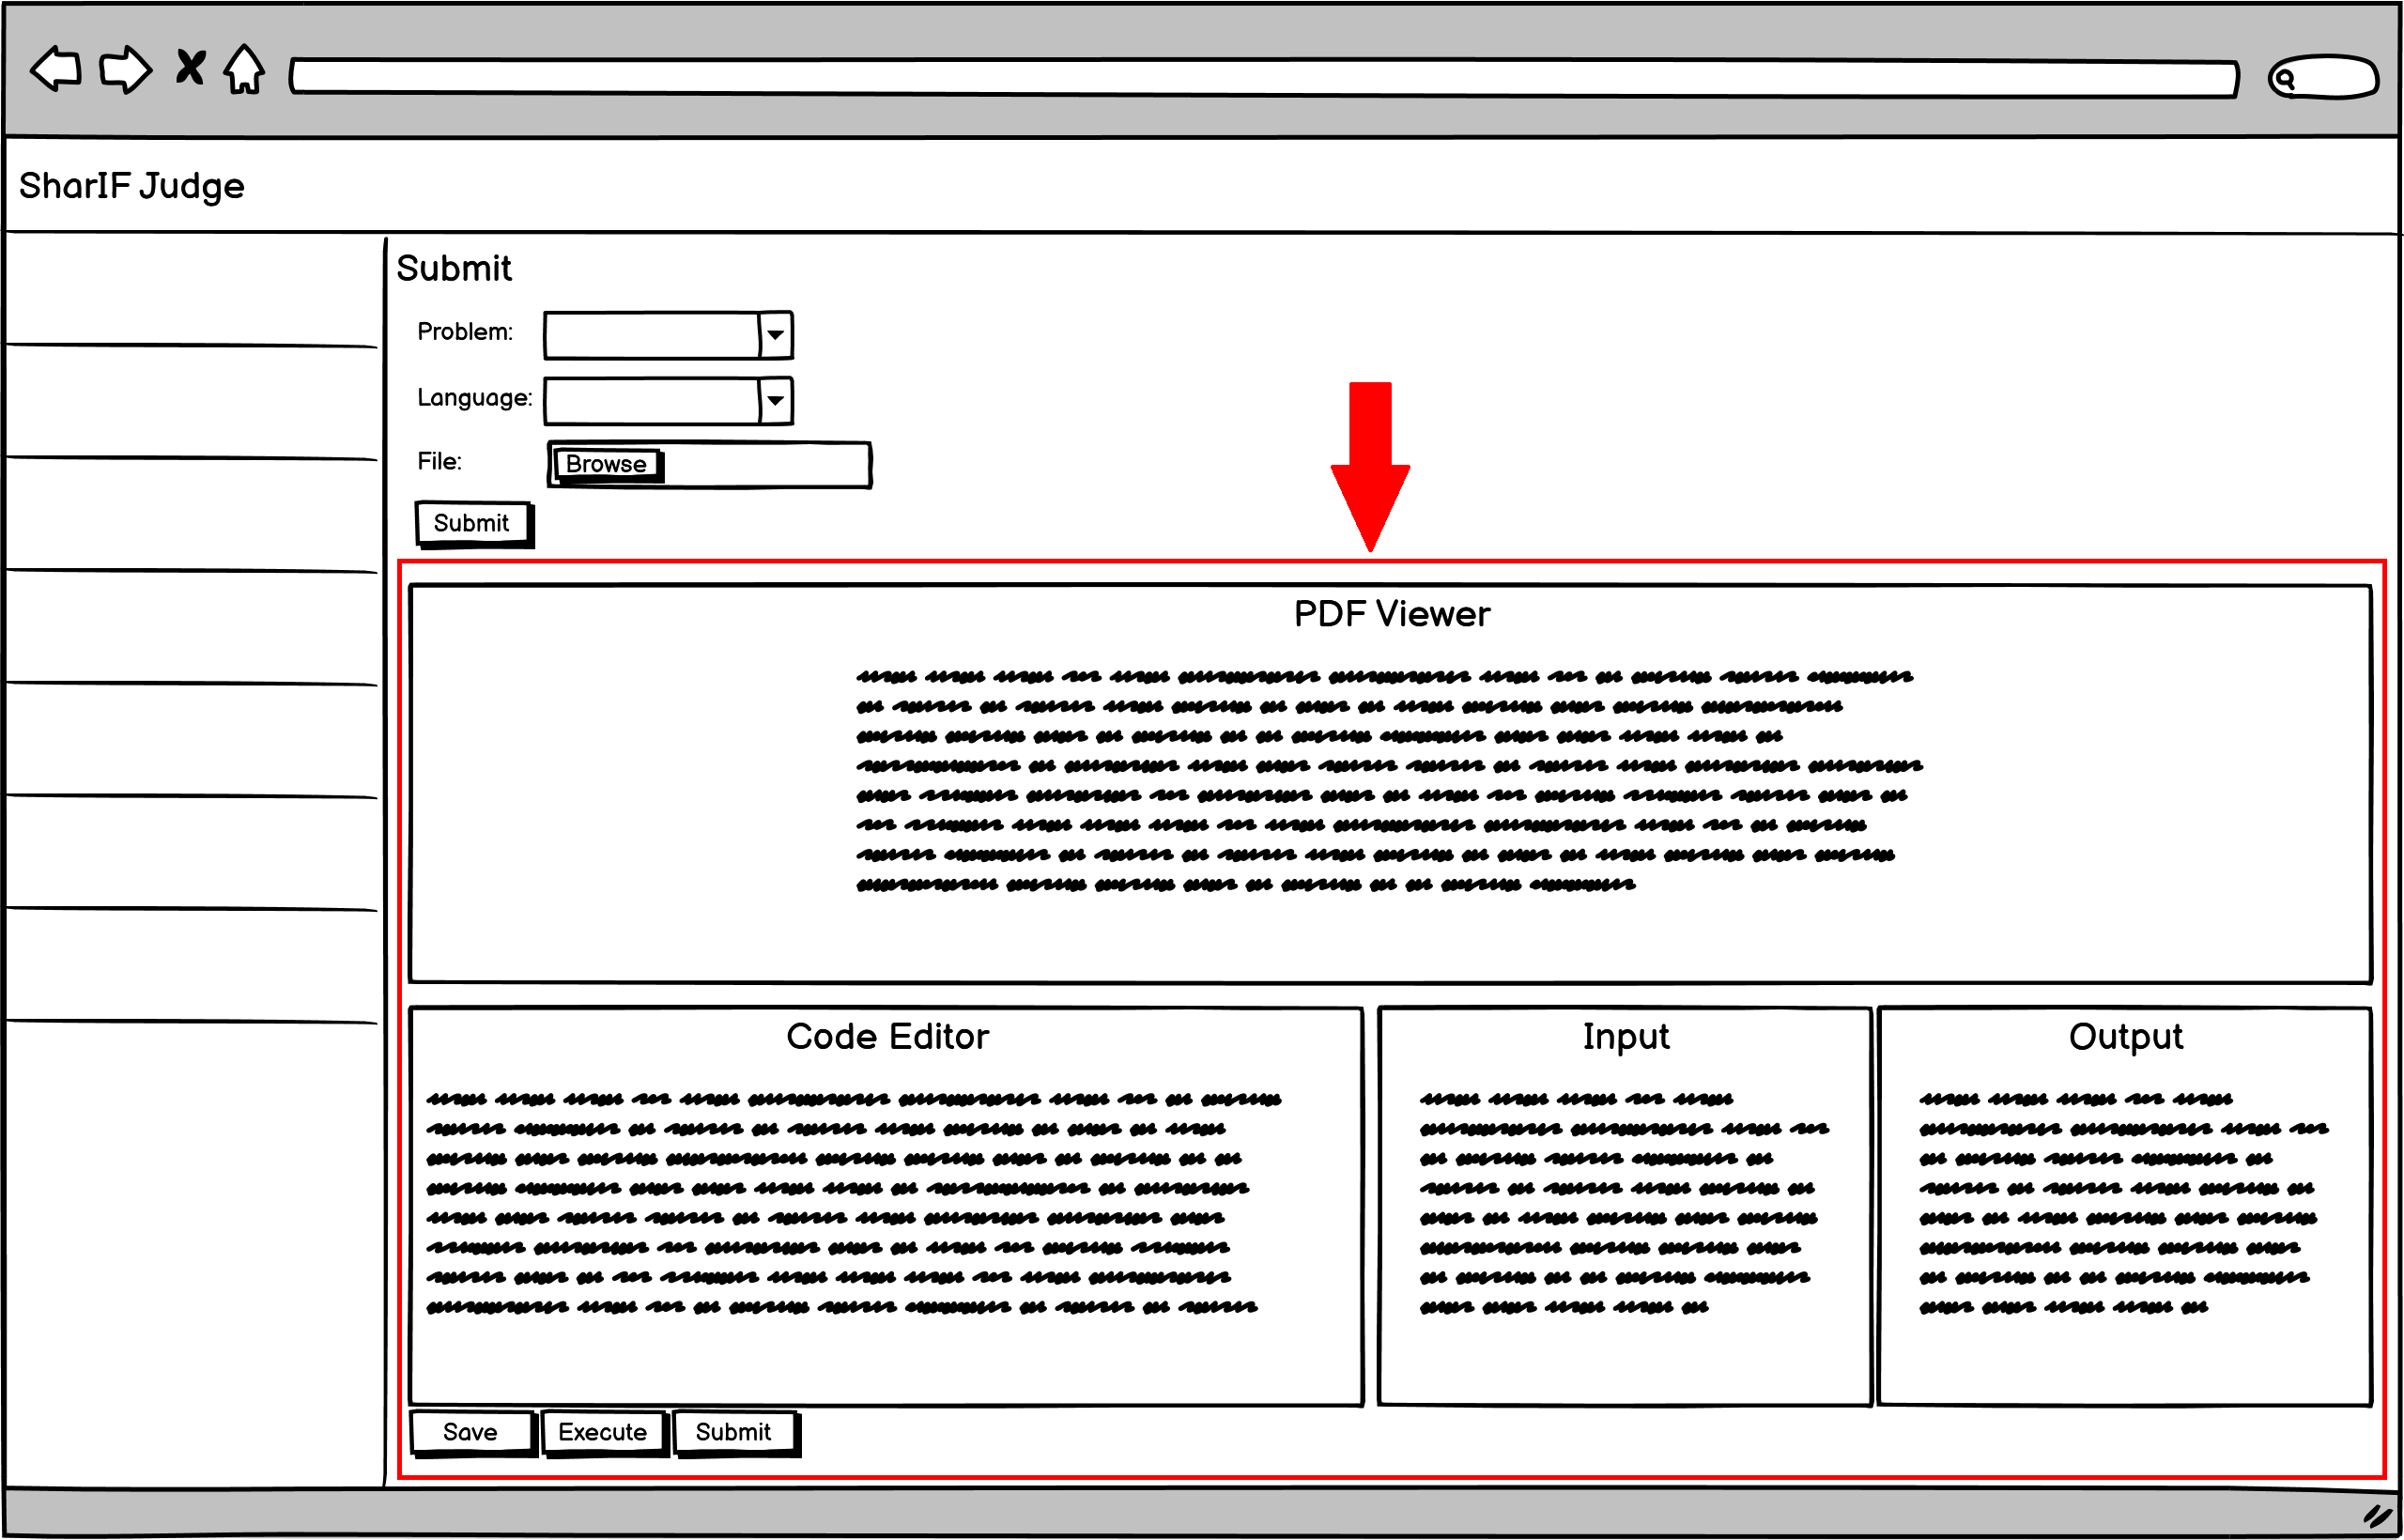
\includegraphics[scale=0.45]{submit_mockup}  
	\caption{Rancangan antarmuka halaman Submit} 
	\label{fig:4:antarmuka} 
\end{figure} 

Seluruh fitur akan diimplementasikan pada halaman Submit. Gambar \ref{fig:4:antarmuka} menunjukkan rancangan antarmuka halaman Submit. Pada halaman Submit sudah terdapat \textit{dropdown} untuk memilih \textit{problem} yang akan dikerjakan, dan bahasa pemrograman yang akan digunakan. Kedua \textit{dropdown} tersebut juga akan digunakan pada fitur yang akan diimplementasikan. \textit{Dropdown} \textit{problem} digunakan untuk menentukan kode yang akan disimpan dan dimuat. Sementara \textit{dropdown} \textit{language} digunakan untuk memilih \textit{mode} \textit{syntax highlighting} pada editor kode.

\section{Menampilkan soal}
\label{sec:4:soal}

SharIF Judge sudah memiliki fitur untuk menyimpan soal dalam bentuk PDF. Untuk melihat soal tersebut, soal harus diunduh terlebih dahulu. Agar pengguna dapat melihat soal secara langsung di halaman Submit, digunakan \textit{library} PDF.js untuk menampilkan \textit{file} PDF soal di halaman Submit.

Untuk menampilkan soal PDF, dilakukan perubahan sebagai berikut:
\begin{itemize}
	\item \textit{Controller} \verb|Assignments|:
    \begin{itemize}
		\item Fungsi \verb|pdf|: \\ Penambahan kondisi untuk mencegah dialog unduh \textit{file}.
    \end{itemize}
    \item \textit{View} \verb|Submit|:
    \begin{itemize}
        \item Penambahan \verb|iframe| untuk menampilkan PDF.js.
    \end{itemize}
\end{itemize}

\section{Mengedit Kode}
\label{sec:4:editor}

Digunakan \textit{library} Ace untuk menambahkan editor kode pada halaman Submit.

Untuk mengimplementasikan editor kode, perlu dilakukan perubahan sebagai berikut:
\begin{itemize}
    \item \textit{View} \verb|Submit|:
    \begin{itemize}
        \item Penambahan \verb|div| sebagai tempat untuk menampilkan editor Ace.
        \item Penambahan \textit{script} untuk konfigurasi Ace.
        \item Penambahan \textit{script} untuk menyesuaikan mode \textit{syntax highlighting} Ace dengan pilihan bahasa pemrograman pada \textit{dropdown}.
    \end{itemize}
\end{itemize}

\section{Menyimpan dan Memuat Kode}
\label{sec:4:simpan}

Seluruh \textit{submission} yang diunggah oleh pengguna pada SharIF Judge akan disimpan pada folder \verb|Assignments| sesuai dengan \textit{assignment} dan \textit{problem} yang dipilih. Kode pada editor kode juga akan disimpan pada folder yang sama sebagai sebuah \textit{file} txt saat pengguna menekan tombol Save. Kode yang sudah tersimpan akan otomatis dimuat pada editor kode saat pengguna memilih \textit{problem} pada \textit{dropdown}.

Untuk menyimpan dan mengambil kode, perlu dilakukan perubahan sebagai berikut:
\begin{itemize}
	\item \textit{Controller} \verb|Submit|:
    \begin{itemize}
		\item Fungsi \verb|save|: \\ Fungsi baru untuk menyimpan kode pada \textit{file} txt.
		\item Fungsi \verb|load|: \\ Fungsi baru untuk memuat kode dari \textit{file} txt.
    \end{itemize}
    \item \textit{View} \verb|Submit|:
    \begin{itemize}
        \item Penambahan \verb|button| untuk menyimpan kode.
        \item Penambahan \textit{script} untuk memanggil fungsi \verb|save| pada \textit{controller} \verb|Submit|. 
        \item Penambahan \textit{script} untuk memanggil fungsi \verb|load| pada \textit{controller} \verb|Submit|. 
    \end{itemize}
\end{itemize}

\section{Menjalankan Kode dengan Tes Kasus}
\label{sec:4:jalan}

Fitur ini memanfaatkan sistem antrean eksekusi kode yang sudah tersedia pada SharIF Judge.
Diperlukan beberapa perubahan agar kode pada editor dapat dimasukkan ke dalam antrean, dijalankan \textit{input} tes kasus, dan \textit{output} dari kode dapat ditampilkan.

Untuk menjalankan kode dengan tes kasus, dilakukan perubahan sebagai berikut:
\begin{itemize}
	\item \verb|tester.sh|:
    \begin{itemize}
        \item Penambahan kondisi untuk menjalankan kode tanpa penilaian dan mencatat hasilnya pada \textit{file} txt.
    \end{itemize}
	\item \textit{Controller} \verb|Submit|:
    \begin{itemize}
        \item Fungsi \verb|_execute|: \\ Fungsi baru untuk memasukkan kode dari editor ke antrean. Fungsi ini dipanggil oleh fungsi \verb|save("execute")|.
        \item Fungsi \verb|get_output|: \\ Fungsi baru untuk memuat hasil eksekusi kode dari \textit{file} txt.
    \end{itemize}
	\item \textit{Controller} \verb|Queueprocess|:
    \begin{itemize}
        \item Fungsi \verb|run|: \\ Penambahan kondisi untuk menjalankan \verb|tester.sh| tanpa penilaian.
    \end{itemize}
    \item \textit{View} \verb|Submit|:
    \begin{itemize}
		\item Penambahan \verb|textarea| untuk \textit{input}.
		\item Penambahan \verb|textarea| untuk \textit{output}.
        \item Penambahan \verb|button| untuk menjalankan kode.
        \item Penambahan \textit{script} untuk memanggil fungsi \verb|save("execute")| pada \textit{controller} \verb|Submit|.
        \item Penambahan \textit{script} untuk memanggil fungsi \verb|get_output| pada \textit{controller} \verb|Submit|.
    \end{itemize}
\end{itemize}

\section{Mengumpulkan Kode Melalui IDE}
\label{sec:4:kumpul}

Fitur ini memanfaatkan fitur \textit{submit} yang sudah tersedia pada SharIF Judge, namun kode yang digunakan adalah kode yang sudah tersimpan pada editor, sebagai ganti dari unggah \textit{file}. 

Untuk mengumpulkan kode dari editor, perlu dilakukan perubahan sebagai berikut:
\begin{itemize}
	\item \textit{Controller} \verb|Submit|:
    \begin{itemize}
		\item Fungsi \verb|_submit|: \\ Fungsi baru untuk mengumpulkan kode. Fungsi ini dipanggil oleh fungsi \verb|save("submit")|.
    \end{itemize}
    \item \textit{View} \verb|Submit|:
    \begin{itemize}
        \item Penambahan \verb|button| untuk mengumpulkan kode.
        \item Penambahan \textit{script} untuk memanggil fungsi \verb|save("submit")| pada \textit{controller} \verb|Submit|. 
    \end{itemize}
\end{itemize}
